%%%%% Set up %%%%%

% Set document style and font size
\documentclass[12pt]{article}\usepackage[]{graphicx}\usepackage[]{color}
%% maxwidth is the original width if it is less than linewidth
%% otherwise use linewidth (to make sure the graphics do not exceed the margin)
\makeatletter
\def\maxwidth{ %
  \ifdim\Gin@nat@width>\linewidth
    \linewidth
  \else
    \Gin@nat@width
  \fi
}
\makeatother

\definecolor{fgcolor}{rgb}{0.345, 0.345, 0.345}
\newcommand{\hlnum}[1]{\textcolor[rgb]{0.686,0.059,0.569}{#1}}%
\newcommand{\hlstr}[1]{\textcolor[rgb]{0.192,0.494,0.8}{#1}}%
\newcommand{\hlcom}[1]{\textcolor[rgb]{0.678,0.584,0.686}{\textit{#1}}}%
\newcommand{\hlopt}[1]{\textcolor[rgb]{0,0,0}{#1}}%
\newcommand{\hlstd}[1]{\textcolor[rgb]{0.345,0.345,0.345}{#1}}%
\newcommand{\hlkwa}[1]{\textcolor[rgb]{0.161,0.373,0.58}{\textbf{#1}}}%
\newcommand{\hlkwb}[1]{\textcolor[rgb]{0.69,0.353,0.396}{#1}}%
\newcommand{\hlkwc}[1]{\textcolor[rgb]{0.333,0.667,0.333}{#1}}%
\newcommand{\hlkwd}[1]{\textcolor[rgb]{0.737,0.353,0.396}{\textbf{#1}}}%
\let\hlipl\hlkwb

\usepackage{framed}
\makeatletter
\newenvironment{kframe}{%
 \def\at@end@of@kframe{}%
 \ifinner\ifhmode%
  \def\at@end@of@kframe{\end{minipage}}%
  \begin{minipage}{\columnwidth}%
 \fi\fi%
 \def\FrameCommand##1{\hskip\@totalleftmargin \hskip-\fboxsep
 \colorbox{shadecolor}{##1}\hskip-\fboxsep
     % There is no \\@totalrightmargin, so:
     \hskip-\linewidth \hskip-\@totalleftmargin \hskip\columnwidth}%
 \MakeFramed {\advance\hsize-\width
   \@totalleftmargin\z@ \linewidth\hsize
   \@setminipage}}%
 {\par\unskip\endMakeFramed%
 \at@end@of@kframe}
\makeatother

\definecolor{shadecolor}{rgb}{.97, .97, .97}
\definecolor{messagecolor}{rgb}{0, 0, 0}
\definecolor{warningcolor}{rgb}{1, 0, 1}
\definecolor{errorcolor}{rgb}{1, 0, 0}
\newenvironment{knitrout}{}{} % an empty environment to be redefined in TeX

\usepackage{alltt}

% File path to resources (style file etc)
\newcommand{\locRepo}{csas-style}

% Style file for DFO Technical Reports
\usepackage{\locRepo/tech-report}

% header-includes from R markdown entry


%%%%% Variables %%%%%

% New definitions: Title, year, report number, authors
% Protect lower case words (i.e., species names) in \Addlcwords{}, in "TechReport.sty"
\newcommand{\trTitle}{Sablefish (\emph{Anoplopoma fimbria}) fork length predictions based on interorbital head length measurements.}
\newcommand{\trYear}{20XX}
\newcommand{\trReportNum}{nnn}
% Optional
\newcommand{\trAuthFootA}{Email: \href{mailto:First.Author@dfo-mpo.gc.ca}{\nolinkurl{First.Author@dfo-mpo.gc.ca}} \textbar{} telephone: (250) 756-5555}
\newcommand{\trAuthsLong}{First. M. Last\textsuperscript{1} and Alex B. Smith\textsuperscript{2}}
\newcommand{\trAuthsBack}{Last, F.M. and Smith, A.B.}

% New definition: Address
\newcommand{\trAddy}{\textsuperscript{1}Pacific Biological Station\\
Fisheries and Oceans Canada, 3190 Hammond Bay Road\\
Nanaimo, British Columbia, V9T 6N7, Canada\\
\textsuperscript{2}Far, far away\\
Another Galaxy}

% Abstract
\newcommand{\trAbstract}{Here is the abstract text. Lorem ipsum dolor sit amet, consectetur adipisicing elit, sed do eiusmod tempor incididunt ut labore et dolore magna aliqua. Ut enim ad minim veniam, quis nostrud exercitation ullamco laboris nisi ut aliquip ex ea commodo consequat. Duis aute irure dolor in reprehenderit in voluptate velit esse cillum dolore eu fugiat nulla pariatur. Excepteur sint occaecat cupidatat non proident, sunt in culpa qui officia deserunt mollit anim id est laborum.}

% Resume (i.e., French abstract)
\newcommand{\trResume}{Voici le résumé. Lorem ipsum dolor sit amet, consectetur adipisicing elit, sed do eiusmod tempor incididunt ut labore et dolore magna aliqua. Ut enim ad minim veniam, quis nostrud exercitation ullamco laboris nisi ut aliquip ex ea commodo consequat. Duis aute irure dolor in reprehenderit in voluptate velit esse cillum dolore eu fugiat nulla pariatur. Excepteur sint occaecat cupidatat non proident, sunt in culpa qui officia deserunt mollit anim id est laborum.}

\newcommand{\trISBN}{}

%%%%% Start %%%%%

% Start the document
\IfFileExists{upquote.sty}{\usepackage{upquote}}{}
\begin{document}

%%%% Front matter %%%%%

% Add the first few pages
\frontmatter

%%%%% Drafts %%%%%

%\linenumbers  % Line numbers
%\onehalfspacing  % Extra space between lines
\renewcommand{\headrulewidth}{0.5pt}  % Header line
\renewcommand{\footrulewidth}{0.5pt}  % footer line
%\pagestyle{fancy}\fancyhead[c]{Draft: Do not cite or circulate}  % Header text

%%%%% Main document %%%%%
\hypertarget{introduction}{%
\section{Introduction}\label{introduction}}

The tag and release study has been conducted annually since 1991.

Tagged fish are recovered mainly in the commercial fishery (trap, trawl, hook and line) and processed at the point of landing through the Dockside Monitoring Program (DMP) currently operated by Archipelago Marine Research (AMR). Tags are also mailed in by individuals or recovered on research trips\ldots.

\hypertarget{methods}{%
\section{Methods}\label{methods}}

Sablefish head morphometric project: Summary Mar 15, 2017.
\begin{enumerate}
\def\labelenumi{\arabic{enumi}.}
\item
  431 Sablefish heads were collected on the 2016 WCVI and WCHG surveys using a trip-wide length stratified sampling protocol.
\item
  We have measured the head dimensions of all 431. In addition, we measured (fork length and head dimensions) and recorded the sex of 7 small sablefish that were collected previously on a salmon survey.
\item
  The 438 heads measured were from fish that ranged from 240-1080 mm fork length. 212 were collected on trip 79190 (WCVI), and 219 were from trip 80378 (WCHG). In addition to measuring the head dimensions as described below, we collected tissue for DNA analysis (small fin clips collected in to 95\% Ethanol) from the first 138 fish measured, and otoliths from every specimen (excluding the 7 small sablefish collected on the salmon survey).
\item
  Table 1 -- Definition of head dimensions measured and instructions for positioning the calipers: MEASUREMENT INSTRUCTIONS FOR POSITIONING CALIPERS Eye Diameter (anterior-posterior diameter of eye socket) Use the outward-facing points of the calipers. Stretch them firmly against the eye socket at the vertical midpoint of the eye InterOrbital Distance (narrowest distance between eye sockets, measured on dorsal surface) Measure at the horizontal midpoint of the eyes on the dorsal surface. Snout length (tip of snout to anterior inner edge of eye socket) Measure from the most forward point/centre of the snout, to the horizontal midpoint of the anterior edge of the eye socket Upper jaw length (tip of snout to the posterior edge of the maxilla) Measure from the most forward point/centre of the snout to the back of the maxilla. Post orbital head length (Posterior inner edge of orbit to dorsal insertion of opercle) Measure from the back of the eye socket (caliper vertically centred), to the `gill cover notch' at the dorsal insertion of the opercle. Hold the operculum taut and measure to the bone underneath the gill cover notch rather than to the flap of skin that forms the notch itself. Post orbital to preoperculum distance (posterior inner edge of orbit to visual insertion point of preopercle)?Need to re-word? Measure from the back of the eye socket (caliper vertically centred), to the preopercle. Lift the preopercle away from the fish slightly so that you can see the preopercle bone underneath the skin. Measure to the point at which you can see the preopercle bone insertion point (this will be underneath the skin and won't necessarily be where the gill slit ends.
\end{enumerate}
\begin{enumerate}
\def\labelenumi{\alph{enumi}.}
\item
  For all measurements except for eye diameter, use the inward-facing points of the calipers
\item
  Hold the calipers perpendicular to the plane of measurement and press firmly against the surface of the fish. Do not press so hard that the flesh of the fish distorts.
\item
  Measure on the right side of the head (if that is not possible, measure on the left side). (Include a note that the measurement was taken on the left, and why)
\item
  Other head dimension measurements tested but not used:
\item
  Head height, but we were not confident that we could measure consistently because some heads were squished, and also it was hard to define exactly where it should be measured.
\end{enumerate}
\begin{enumerate}
\def\labelenumi{\roman{enumi}.}
\setcounter{enumi}{1}

\item
  `Head length' (horizontal distance from tip of snout through midline of head to posterior margin of cleithrum, measured on dorsal surface) as described in the literature -- we rejected this measurement because it was not clear as to where the cleithrum was located on the outside of the sablefish head.
\item
  Pelvic or pectoral fin length -- this did not work very well - it was unclear as to where the measurement should be taken -- the rays just get thinner and thinner until it is just membrane.
\item
  Posterior orbit to anterior part of the terminus of the cleithrum (the bone that forms the posterior portion of the gill chamber. Tried measuring to the anterior part of the terminus (triangular, most dorsal notch) (lifted the operculum, measured to the bone underneath the pointy part of the operculum. But it moved around a lot (maybe in an intact fish this would be a good landmark but with nothing to hold it still, it didn't seem to work particularly well for this purpose. The other landmarks on the head (including the part of the cleithrum under the gill cover notch) were more supported by the skull.
\item
  Snout to the anterior terminus of the cleithrum on the ventral side, but this was no good (too hard to be consistent in measuring).
\end{enumerate}
\begin{enumerate}
\def\labelenumi{\arabic{enumi}.}
\setcounter{enumi}{4}
\item
  After measuring 137 fish, we looked at the preliminary data (excel scatter plots showing dimension vs fork length, and the correlation coefficients), and decided that a) we had enough tissue for the development of a genetic sex determination test (so wouldn't collect any more tissue going forward), and that b) we would drop the `post orbital head length measurement for the remaining fish, in order to save time. The reason being, it was not as easy to measure (calipers - did not work as well for big measurements, end points were not easy to define, and is not as easily repeatable as the other dimensions). Also the operculum was sometimes cut off (and therefore not measurable) and we also suspect that the operculum would be cut off in commercially caught fish when they are processing.
\item
  We also flagged the `eye diameter' measurement as being weak (due to questionable repeatability) but carried on measuring this dimension on the remaining fish for completeness.
\item
  A total of 438 heads were measured but each dimension measured had a slightly different sample size. Reasons for the missing measurements were noted in the sampling comments (for example, on occasion we forgot to measure a dimension, could not measure a dimension because the fish was damaged; we also started measuring the `post orbital to preoperculum distance' only after the first 13 fish). If the right side of the fish was damaged so that a measurement wasn't possible, we measured on the left side. We noted this, but these measurements are included in the dataset.
\item
  Each measurement was ranked in terms of `Ease of Use' and `Repeatability' (Table 2).
\end{enumerate}
\clearpage

\hypertarget{results}{%
\section{Results}\label{results}}

A simple linear regression was calculated to predict sablefish fork length based on interorbital head length.

\#Tables


\begin{table}[!h]

\caption{\label{tab:table1}Definition of head dimensions measured and instructions for positioning the calipers.}
\fontsize{8}{10}\selectfont
\begin{tabular}[t]{ll}
\toprule
MEASUREMENT \vphantom{3} \vphantom{2} \vphantom{1} & INSTRUCTIONS.FOR.POSITIONING.CALIPERS\\
\midrule
Eye Diameter (anterior-posterior diameter of eye socket) & Use the outward-facing points of the calipers. Stretch them firmly against the eye socket at the vertical midpoint of the eye\\
 & \\
InterOrbital Distance (narrowest distance between eye sockets, measured on dorsal surface) & Measure at the horizontal midpoint of the eyes on the dorsal surface.\\
 & \\
Snout length (tip of snout to anterior inner edge of eye socket) & Measure from the most forward point/centre of the snout, to the horizontal midpoint of the anterior edge of the eye socket\\
 & \\
Upper jaw length (tip of snout to the posterior edge of the maxilla) & Measure from the most forward point/centre of the snout to the back of the maxilla.\\
 & \\
Post orbital head length (Posterior inner edge of orbit to dorsal insertion of opercle) & Measure from the back of the eye socket (caliper vertically centred), to the ‘gill cover notch’ at the dorsal insertion of the opercle.  Hold the operculum taut and measure to the bone underneath the gill cover notch rather than to the flap of skin that forms the notch itself.\\
Post orbital to preoperculum distance (posterior inner edge of orbit to visual insertion point of preopercle)?Need to re-word? & Measure from the back of the eye socket (caliper vertically centred), to the preopercle.  Lift the preopercle away from the fish slightly so that you can see the preopercle bone underneath the skin. Measure to the point at which you can see the preopercle bone insertion point (this will be underneath the skin and won’t necessarily be where the gill slit ends.\\
\bottomrule
\end{tabular}
\end{table}

\begin{table}[!h]

\caption{\label{tab:table2}Ease of Use and Repeatability Considerations for each Measurement.}
\fontsize{8}{10}\selectfont
\begin{tabular}[t]{lrrlrl}
\toprule
Type & N & R & Ease.of.use & Repeatability & Considerations\\
\midrule
Snout length & 437 & 0.976 & 4 & 5 & Bony part; can measure on right or left side\\
 &  &  &  &  & Must ensure caliper is in centre of snout\\
\hline
Upper jaw length & 437 & 0.973 & 3 & 4 & Bony part; can measure on right or left side\\
 &  &  & -ÿÿÿÿÿÿÿÿÿ b &  & Electronic Calipers tended to malfunction when longer measurements attempted; had to use manual calipers for >15cm distances; somewhat awkward to measure.\\
 &  &  &  &  & The end of the maxilla can be hard to define.\\
 &  &  &  &  & Must ensure caliper is in center of snout\\
Interorbital distance & 437 & 0.971 & 5 & 5 & Bony part;  Easy to define where to hold calipers; so far there has been no reason (eg damage) to not include this measurement\\
Post orbital to pre-operculum & 426 & 0.965 & 4 & 5 & Bony part; can measure on right or left side\\
 &  &  &  &  & Maybe need to improve definition of instruction of where to hold caliper on pre-operculum\\
Post orbital head length & 130 & 0.956 & 3 & 2 & Can measure on right or left side\\
 &  &  &  &  & Operculum was cut off on some fish, likely to be cut off on commercially caught fish. Electronic Calipers tended to malfunction when longer measurements attempted; had to use manual calipers for >15 cm distances\\
 &  &  &  &  & \\
Eye diameter & 438 & 0.938 & 3 & 2 & Easy to define where to hold the calipers in the eye socket, but the tissue is soft/stretchy so its difficult to know how hard to press against the flesh; can measure on right or left side\\
 &  &  &  &  & Uses the outside rather than the inside of the calipers (? slower); Soft tissue so repeatability is questionable; somewhat awkward to measure\\
\bottomrule
\end{tabular}
\end{table}
\hypertarget{figures}{%
\section{Figures}\label{figures}}


\begin{figure}[htb]

{\centering \pdftooltip{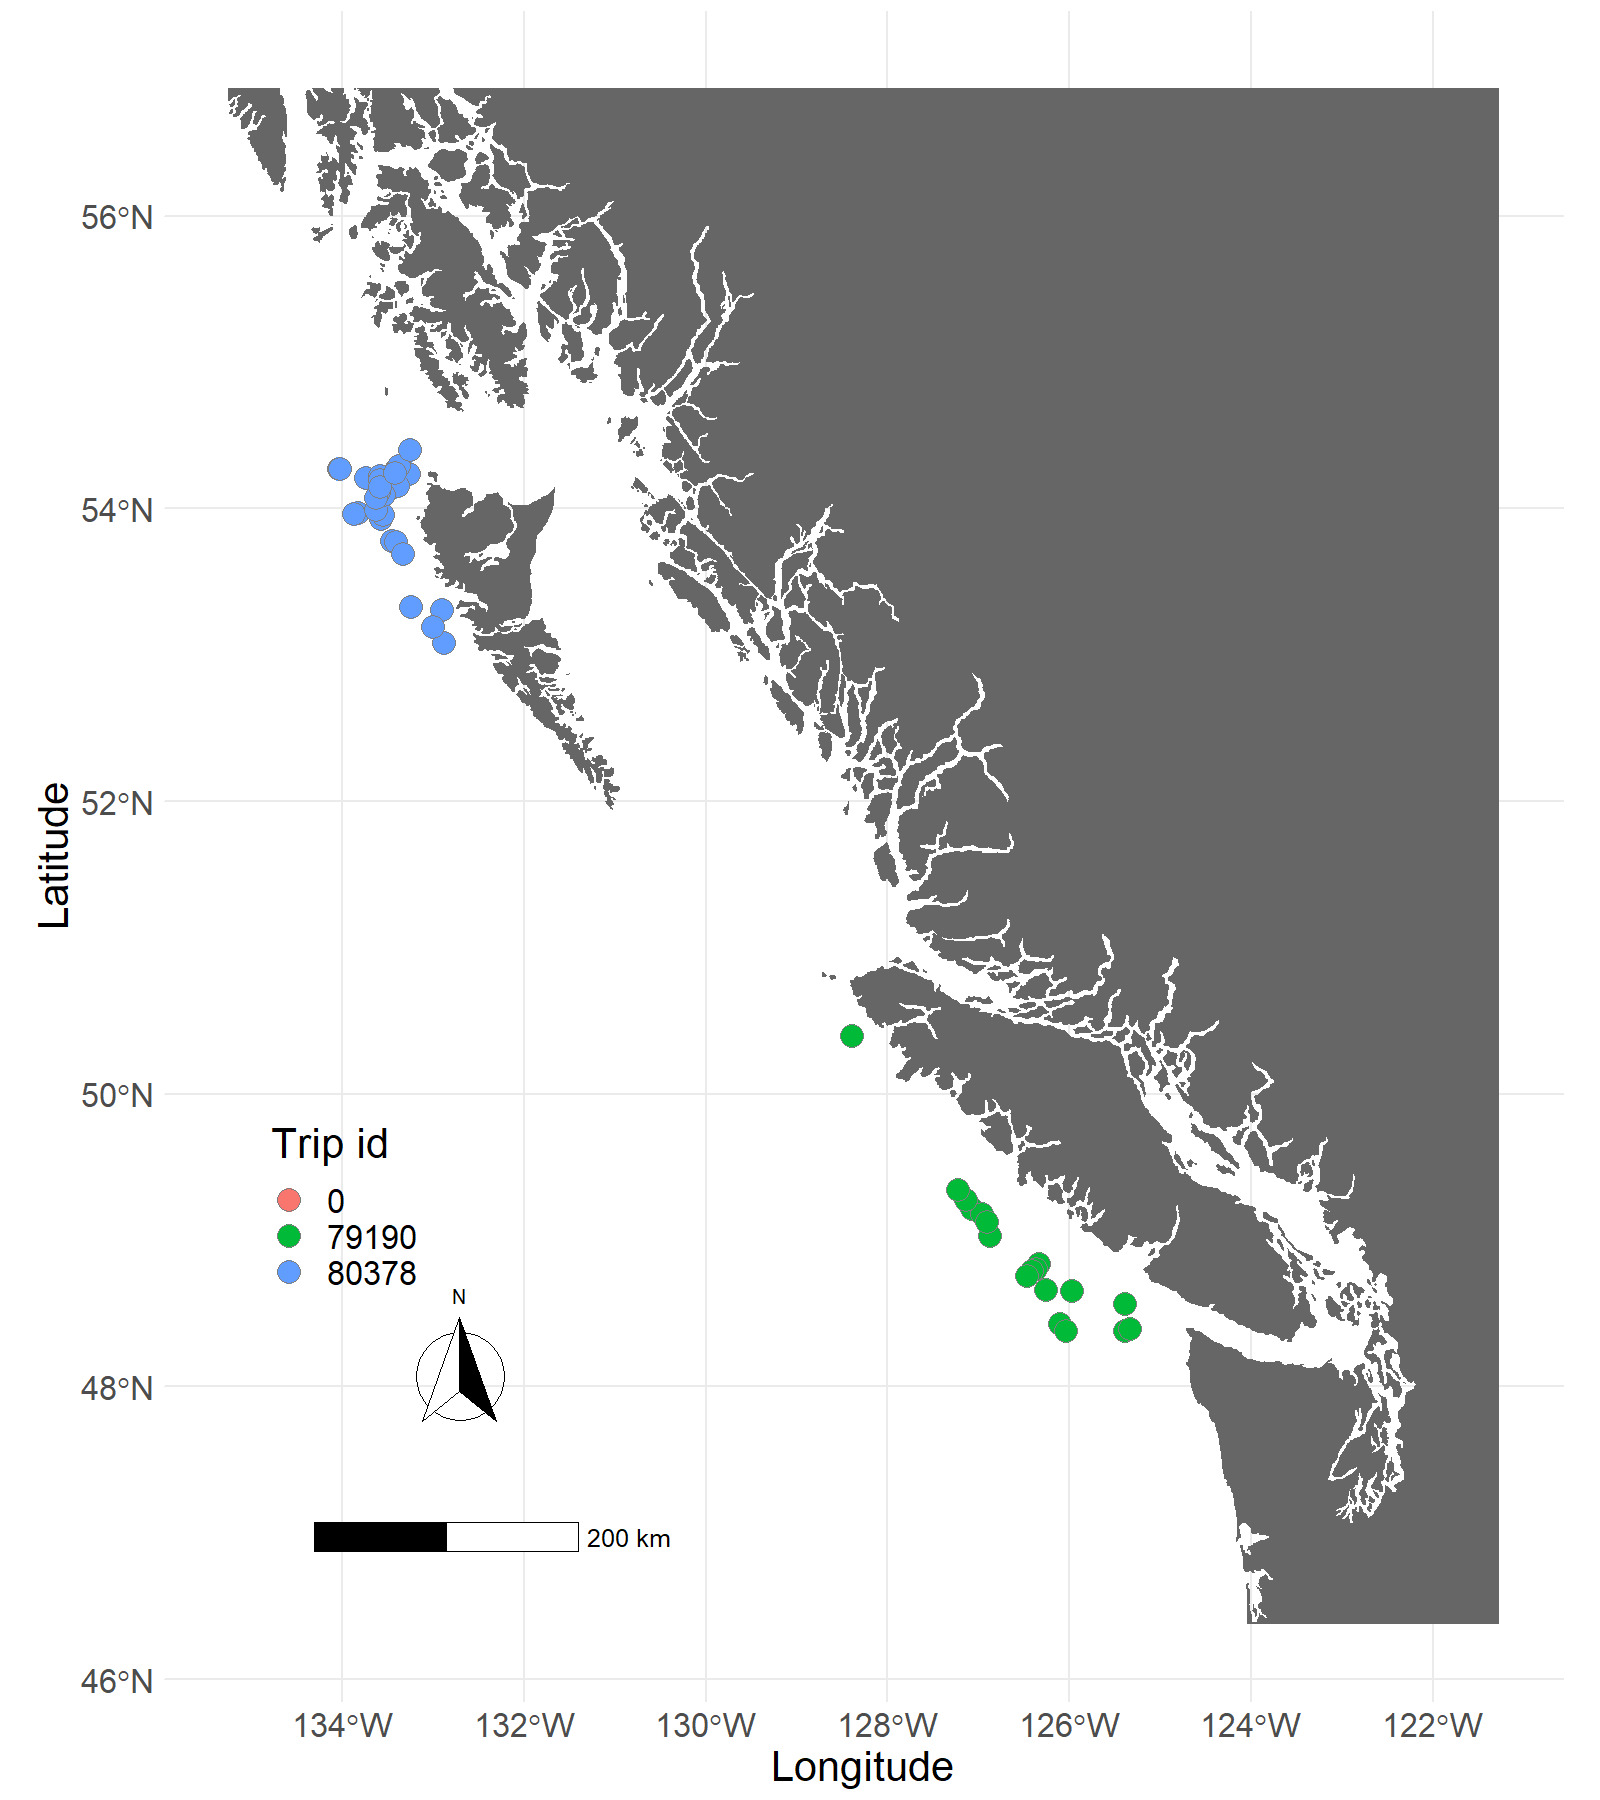
\includegraphics[width=6in]{C:/github/headresults/figures/Figure1}}{Figure \ref{fig:figure1}} 

}

\caption{Upper jaw measurement.}\label{fig:figure1}
\end{figure}

\begin{figure}[htb]

{\centering \pdftooltip{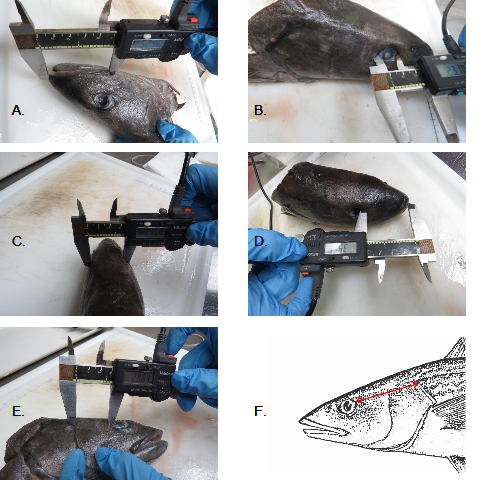
\includegraphics[width=6in]{C:/github/headresults/figures/Figure2}}{Figure \ref{fig:figure2}} 

}

\caption{Eye diameter measurement.}\label{fig:figure2}
\end{figure}

\begin{figure}[htb]

{\centering \pdftooltip{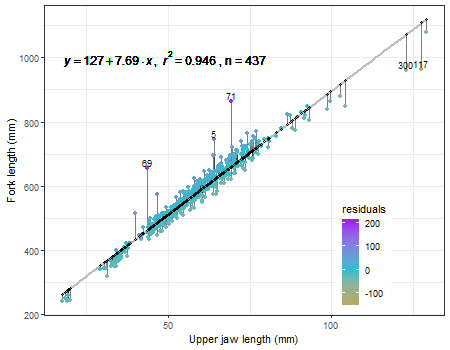
\includegraphics[width=6in]{C:/github/headresults/figures/Figure3}}{Figure \ref{fig:figure3}} 

}

\caption{Interorbital measurement.}\label{fig:figure3}
\end{figure}

\begin{figure}[htb]

{\centering \pdftooltip{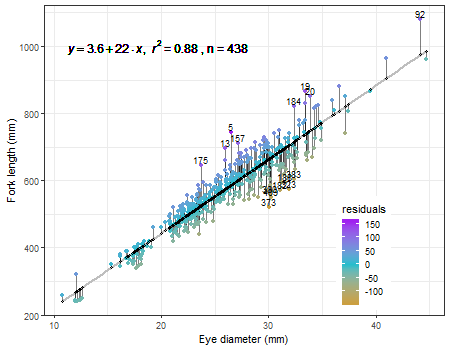
\includegraphics[width=6in]{C:/github/headresults/figures/Figure4}}{Figure \ref{fig:figure4}} 

}

\caption{Post orbital to preoperculum length measurement.}\label{fig:figure4}
\end{figure}

\begin{figure}[htb]

{\centering \pdftooltip{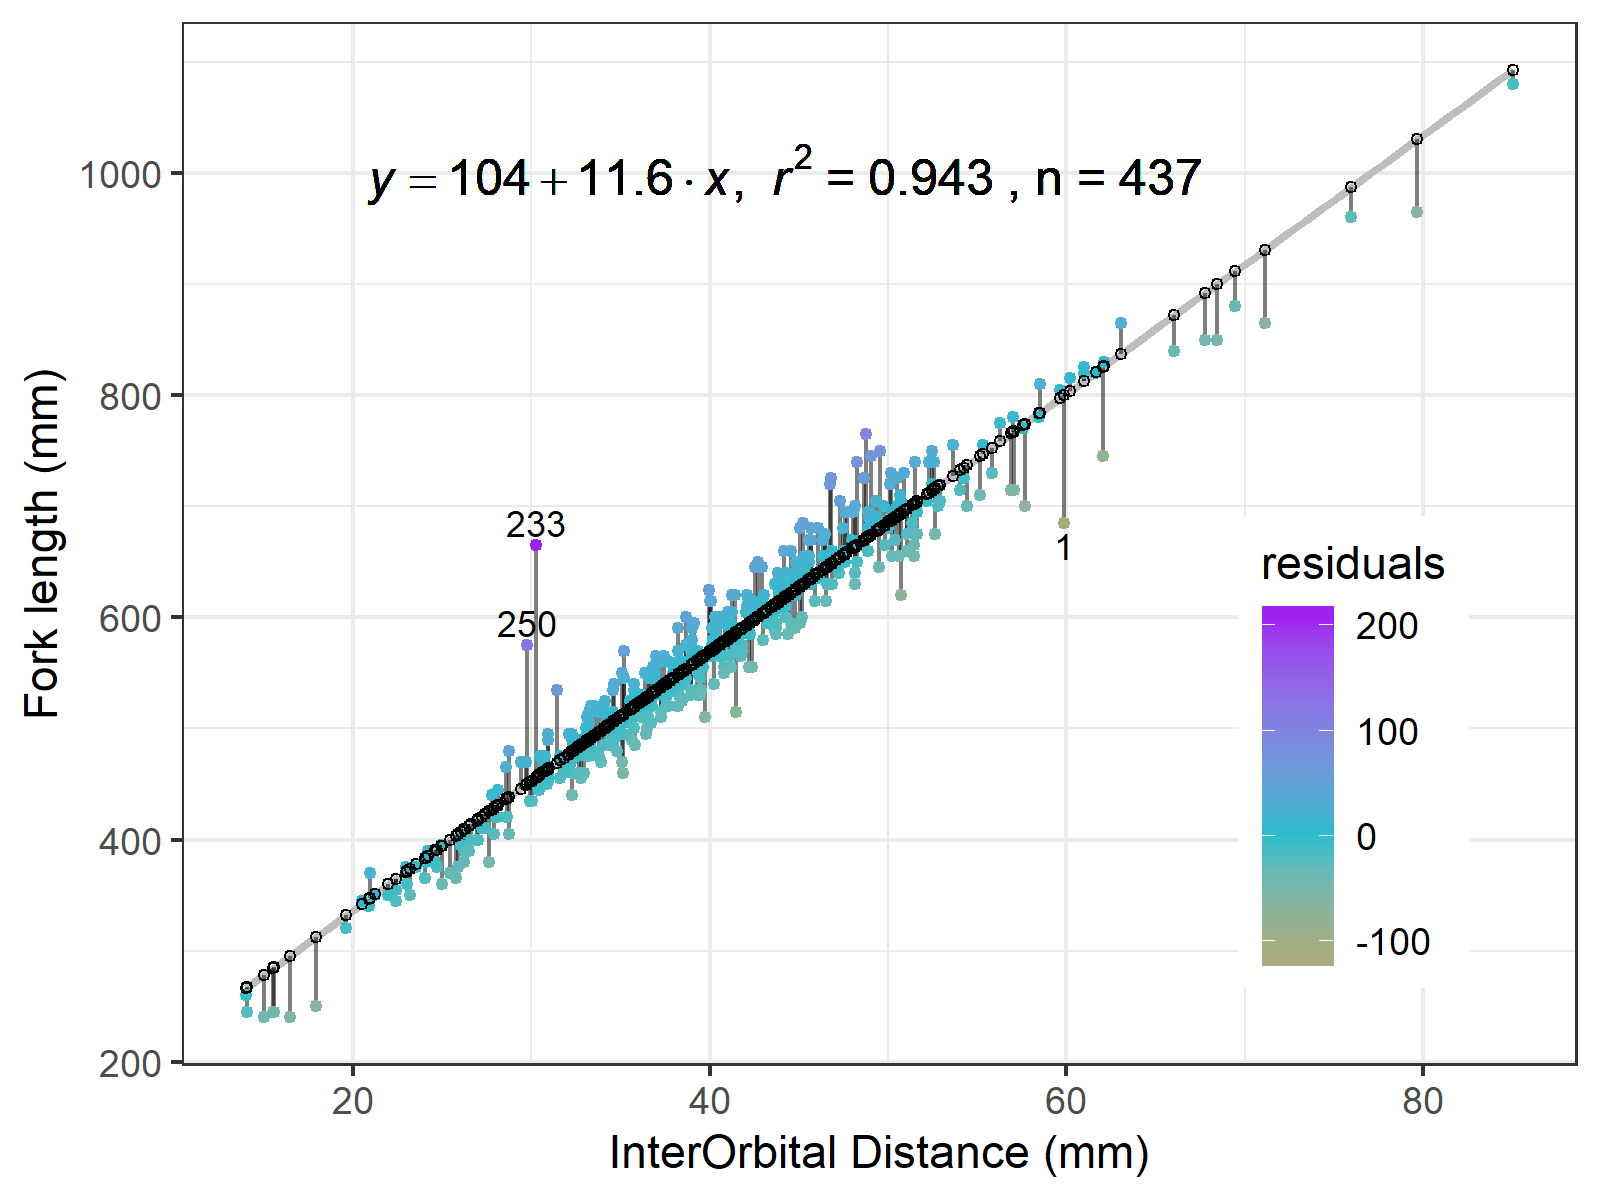
\includegraphics[width=6in]{C:/github/headresults/figures/Figure5}}{Figure \ref{fig:figure5}} 

}

\caption{Post orbital head length.}\label{fig:figure5}
\end{figure}

\begin{figure}[htb]

{\centering \pdftooltip{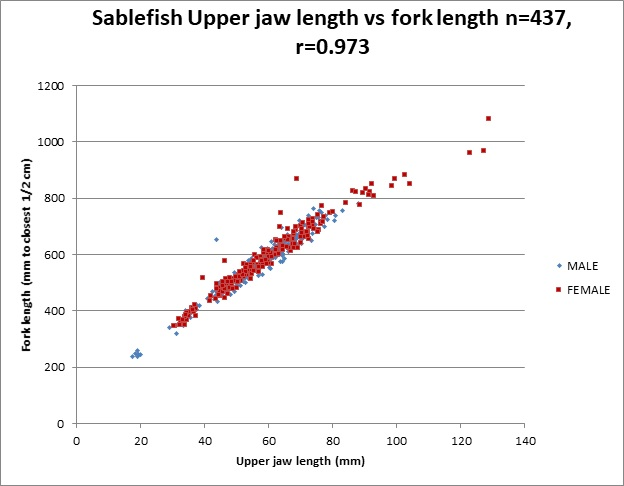
\includegraphics[width=6in]{C:/github/headresults/figures/Figure1a}}{Figure \ref{fig:figure6}} 

}

\caption{Scatterplot upper jaw vs fork length.}\label{fig:figure6}
\end{figure}

\begin{figure}[htb]

{\centering \pdftooltip{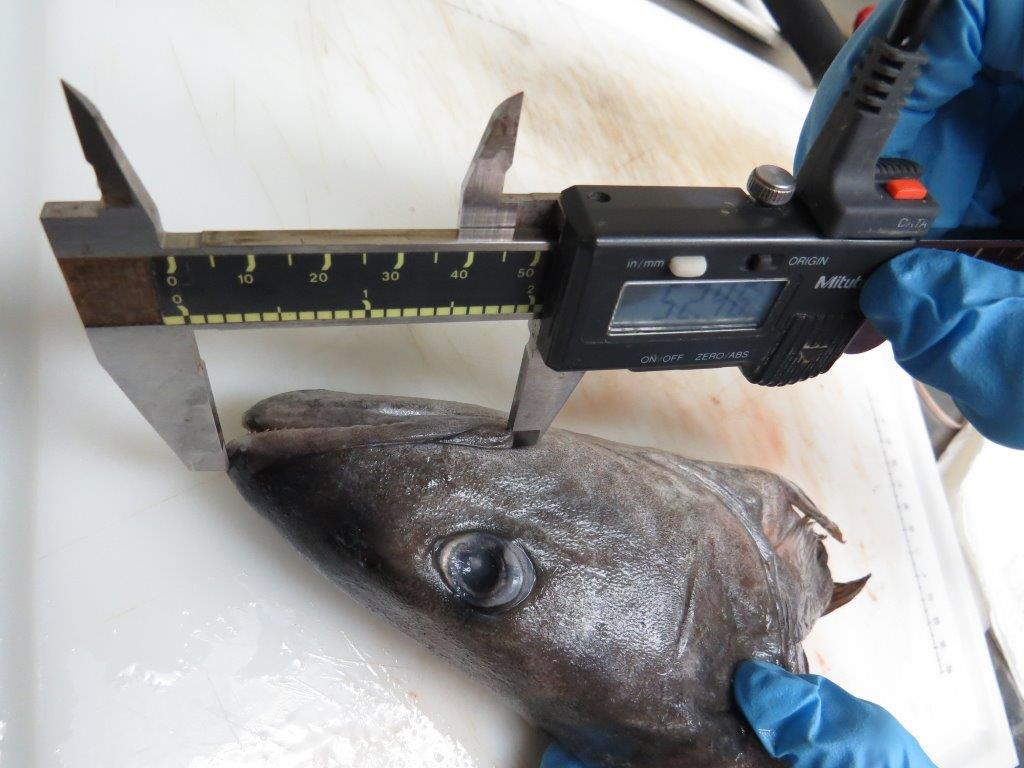
\includegraphics[width=6in]{C:/github/headresults/figures/Figure2a}}{Figure \ref{fig:figure7}} 

}

\caption{Scatterplot eye diameter vs fork length.}\label{fig:figure7}
\end{figure}

\begin{figure}[htb]

{\centering \pdftooltip{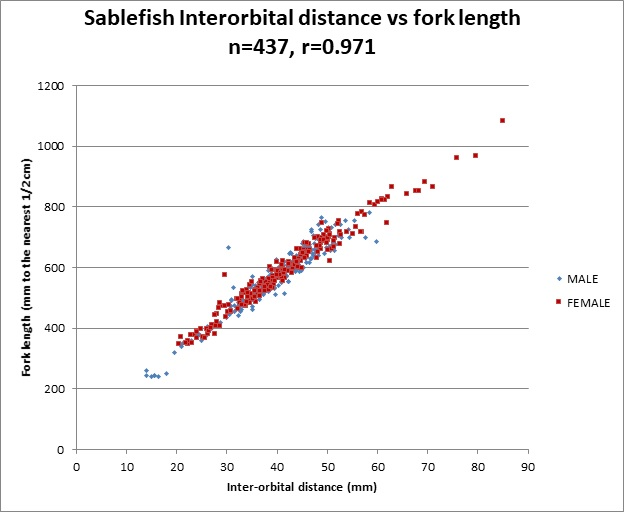
\includegraphics[width=6in]{C:/github/headresults/figures/Figure3a}}{Figure \ref{fig:figure8}} 

}

\caption{Scatterplot interorbital vs fork length.}\label{fig:figure8}
\end{figure}

\begin{figure}[htb]

{\centering \pdftooltip{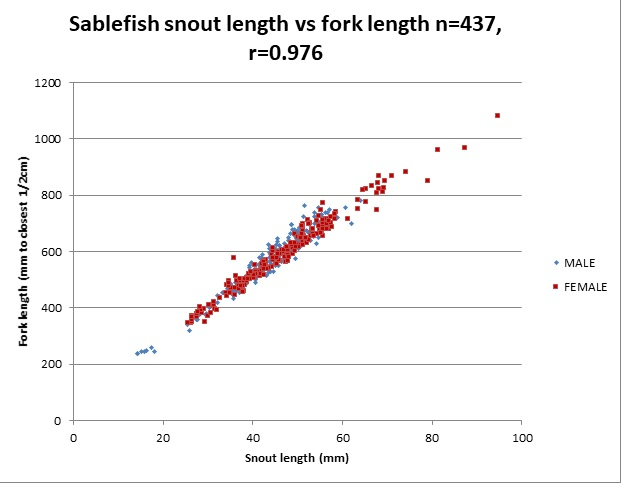
\includegraphics[width=6in]{C:/github/headresults/figures/Figure4a}}{Figure \ref{fig:figure9}} 

}

\caption{Scatterplot post orbital to preoperculum vs fork length.}\label{fig:figure9}
\end{figure}

\begin{figure}[htb]

{\centering \pdftooltip{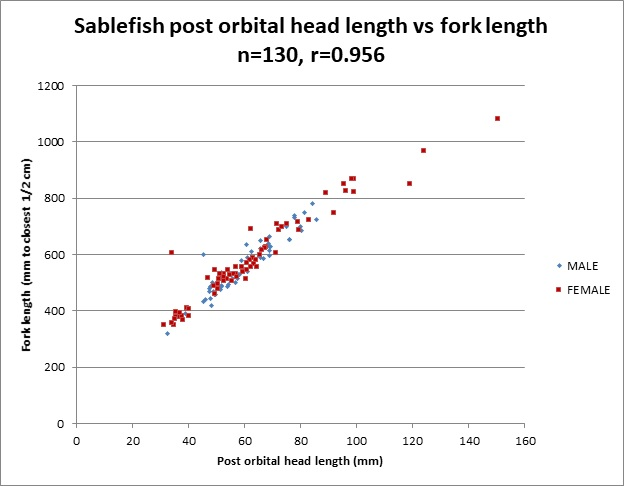
\includegraphics[width=6in]{C:/github/headresults/figures/Figure5a}}{Figure \ref{fig:figure10}} 

}

\caption{Scatterplot post orbital vs fork length.}\label{fig:figure10}
\end{figure}
\end{document}
